\section{Sensor Testing and Results}\label{sec:results}

Since gas sensors are inherently inaccurate due to their manufacturing processes and biases, each sensor had to be calibrated by graphing the output of each sensor compared to the known gas in the testing environment. The testing environments consisted of 1.0 liter sealed containers with the sensor inserted into one end and a septum for needles inserted in the other as illustrated in Fig. \ref{fig:sensor}. The 1.0 liter volume simplified the calculations in parts-per-million (ppm) and each gas was introduced to the environment via a syringe and needle.

\begin{figure}
	\centering
	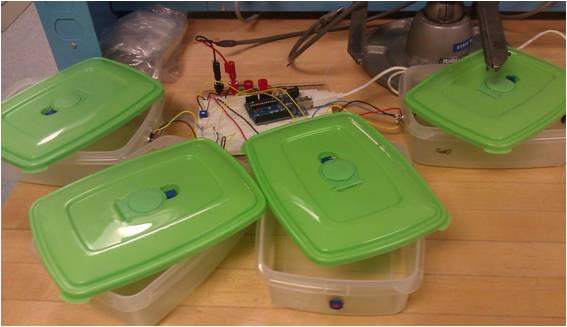
\includegraphics[width=0.5\textwidth]{./pictures/sensor.jpg}
	\caption{Testing environments (from left to right): MQ-4, MQ-6, MQ-7, and MQ-8 sensors.}
	\label{fig:sensor}
\end{figure}

By comparing the sensor output (x-axis) to the known concentration of gas in the testing environment (y-axis), a curve is formed, which can be best fit to an exponential curve by focusing the comparison on moderately to severely dangerous gas concentrations, which is approximately 2,000 to 10,000 ppm. The best fit equation for the most accurate test is used in software to correct the sensor output to the most accurate output for transmission to the operator through the OCU. Fig. \ref{fig:sensor-testing} displays the graph for the MQ-4 (Methane) sensor along with the graphs for MQ-6 (Liquefied Petroleum Gas), MQ-7 (Carbon Monoxide), and MQ-8 (Hydrogen) sensors.

\begin{figure}
	\centering
	{\subfloat[Methane]{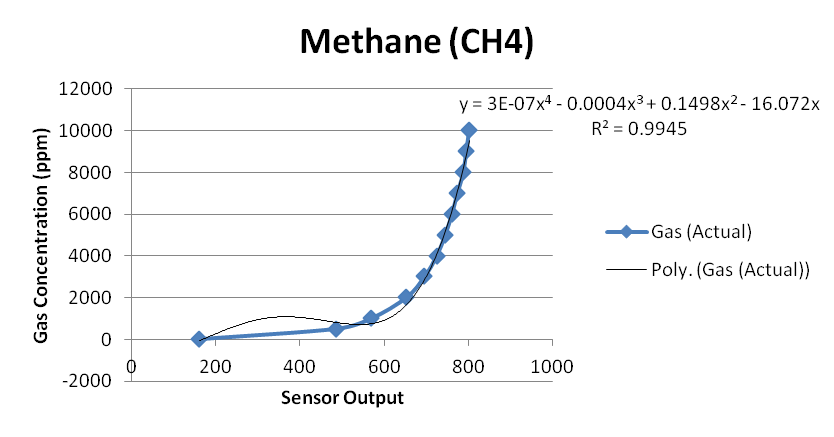
\includegraphics[width=0.4\textwidth]{./pictures/methane1.png}\label{fig:methane1}} \\
	%\hfil
	\subfloat[LPG]{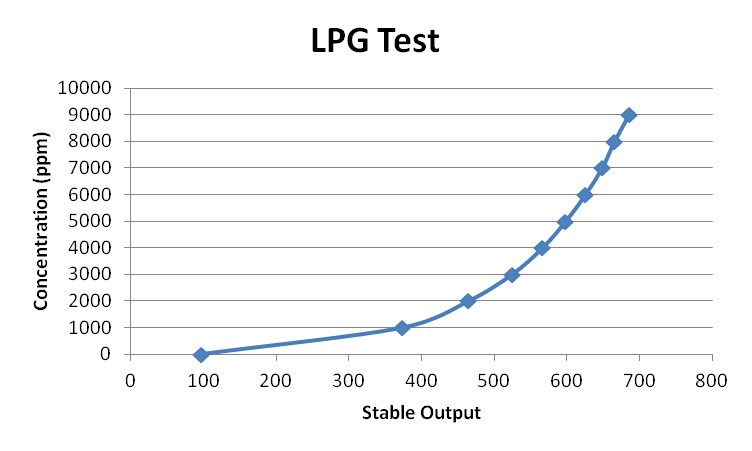
\includegraphics[width=0.4\textwidth]{./pictures/lpg.png}\label{fig:lpg}} \\
	%\hfil
	\subfloat[CO]{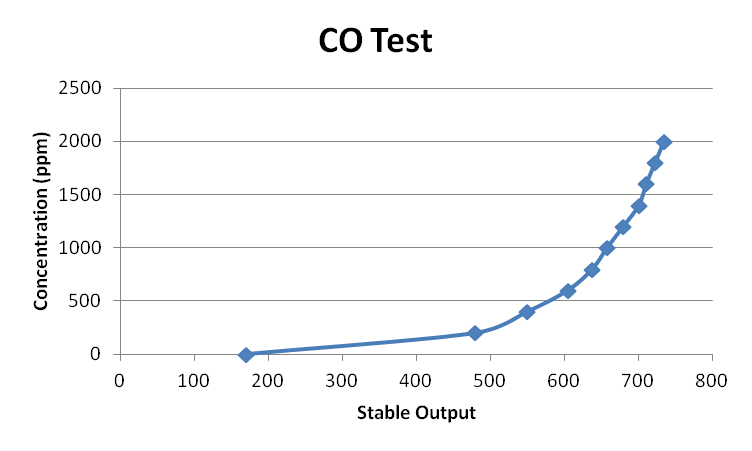
\includegraphics[width=0.4\textwidth]{./pictures/co.png}\label{fig:co}} \\
	%\hfil
	\subfloat[Hydrogen]{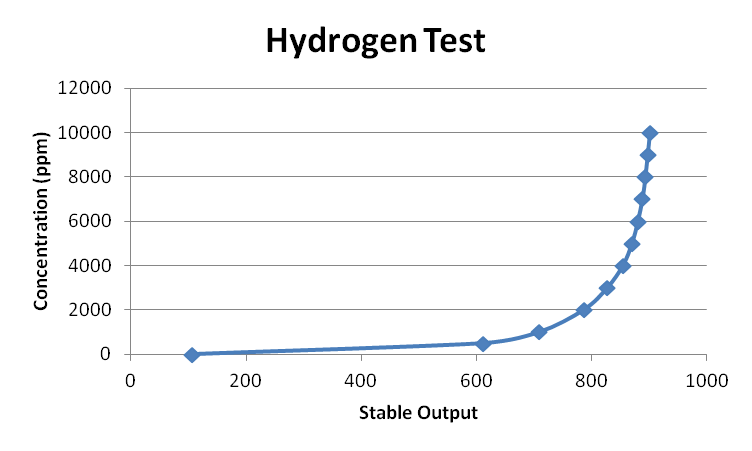
\includegraphics[width=0.4\textwidth]{./pictures/hydrogen.png}\label{fig:hydrogen}}}
	\caption{Dangerous gases and liquids testing.}
	\label{fig:sensor-testing}
\end{figure}

Using the correction equations in the code with the given sensor outputs, the final results fairly closely match the expected concentrations. Granted they are not extremely accurate, but the corrected outputs will be able to discern the difference between a safe and a dangerous environment. Table 1 details the MQ-4 sensor results and the results for the MQ-6, MQ-7, and MQ-8 are detailed in Annex 4, Tables 2 – 4 respectively.
